\section{Results}\label{sec:results}

% Each recording made with the Otii software samples power draw in watts 10,000 times per second. For every unique configuration of RPi, OS, and Python version, 10 recordings are made -- one for each benchmarking run. Average power draw and the runtime in seconds are extracted from each individual recording, with energy consumption in joules being calculated immediately as well. These results are then written to a CSV file uniquely named by the three parameters, e.g. \texttt{results\_RPi3B+\_Alpine\_python3.9.csv}, such that every CSV file contains the results for the 10 recordings made for that configuration. The CSV files can all be found in the repository.



\begin{figure}[t]
    \centering
    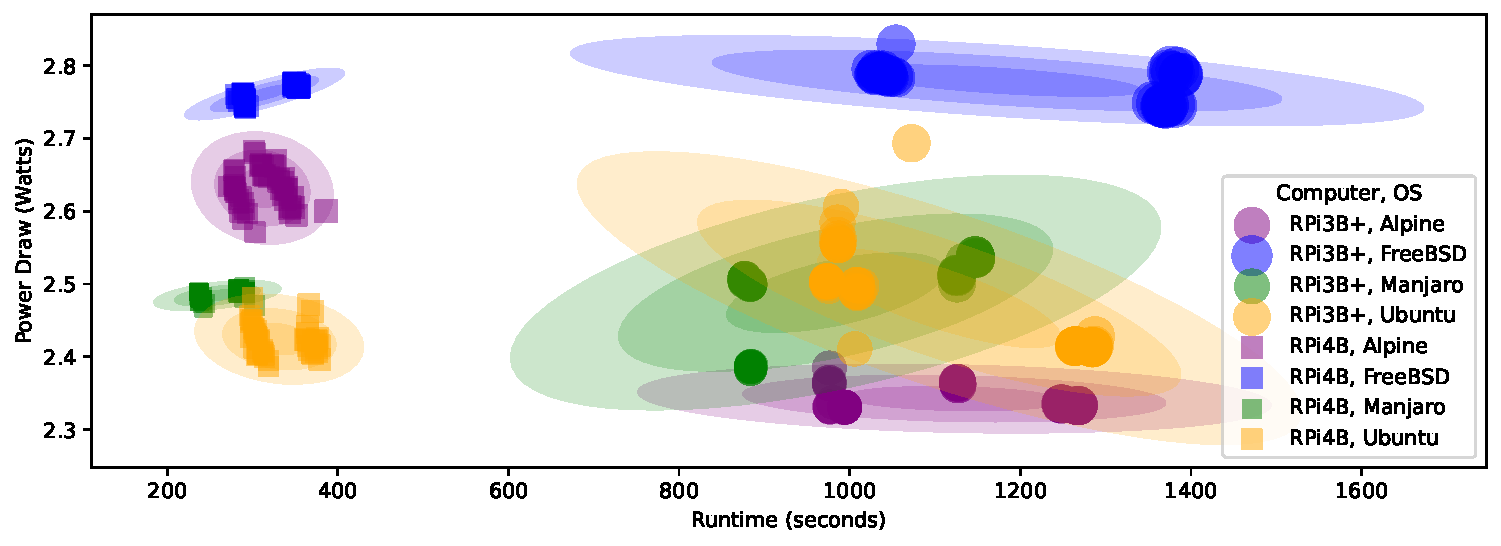
\includegraphics[width=1\textwidth]{images/P_t_E_bagplot.pdf}
    \caption{.}
    \label{fig:results}
\end{figure}

\autoref{fig:results} illustrates the results of our measurements as a scatter plot.
The x-axis shows the runtime of a \gls{pyperformance} benchmark in seconds.
The y-axis lists the measured power draw in Watts.
Each element in the scatter plot corresponds to the power draw and runtime of a benchmark in a certain configuration.
Shapes of elements (squares to the left and circles to the right) denote the \gls{sut} on which a benchmark is executed.
Color of elements corresponds to the respective \gls{os}.
The size of each element is proportional to the energy consumption of a benchmark execution, i.e., the product of power draw and runtime.


Note, for reporting we use the following notation:
$q_{0}$ denotes the minimum,
$q_{1}$ the 25\textsuperscript{th} quartile,
$q_{2}$ the median,
$q_{3}$ the 75\textsuperscript{th} quartile,
$q_{4}$ the maximum,
$\mu$ is the arithmetic mean (we use average and arithmetic mean synonymously),
and the standard deviation is denoted by $\sigma$.

It can be seen that benchmarks run faster on the \toolname{Raspberry Pi 4B}
($q_{0} \approx 237.13\unit{\second}$,
$q_{1} \approx 283.86\unit{\second}$,
$q_{2} \approx 297.51\unit{\second}$,
$q_{3} \approx 338.6\unit{\second}$,
$q_{4} \approx 386.52\unit{\second}$,
$\mu \approx 303.95\unit{\second}$,
$\sigma \approx39.66$)
compared to a \toolname{Raspberry Pi 3B+}
($q_{0} \approx 876.03\unit{\second}$,
$q_{1} \approx 984.18\unit{\second}$,
$q_{2} \approx 1042.14\unit{\second}$,
$q_{3} \approx 1253.09\unit{\second}$,
$q_{4} \approx 1388.55\unit{\second}$,
$\mu \approx 1096.04\unit{\second}$,
$\sigma \approx 155.79$).
The longest runtime ($23\unit{\minute}:08\unit{\second}$) of a benchmark is on a \toolname{Raspberry Pi 3B+} with \projname{FreeBSD} and \cpv{10} whereas the fastest ($3\unit{\minute}:57\unit{\second}$) is on a \toolname{Raspberry Pi 4B} with \projname{Manjaro} and \cpv{11}.
However, note that on average, which is denoted by the centers of the ellipses, benchmark runtimes differ on the \gls{os}.
For example, on a \toolname{Raspberry Pi 4B} benchmarks over all versions of \python run fastest on \projname{Manjaro} ($\mu \approx 4\unit{\minute}:18\unit{\second}$) followed by \projname{Apline} ($\mu \approx 5\unit{\minute}:12\unit{\second}$), \projname{FreeBSD} ($\mu \approx 5\unit{\minute}:14\unit{\second}$) and \projname{Ubuntu} ($\mu \approx 5\unit{\minute}:31\unit{\second}$).
That is ca. $1\unit{\minute}:10\unit{\second}$ difference between the ``fastest'' and the ``slowest'' \gls{os}.
On the \toolname{Raspberry Pi 3B+} the order of \glspl{os} with respect to runtimes of benchmarks is different though.
Here, the benchmarks over all versions of \python run fastest on \projname{Manjaro} ($\mu \approx 16\unit{\minute}:23\unit{\second}$) followed by \projname{Ubuntu} ($\mu \approx 18\unit{\minute}:24\unit{\second}$),
\projname{Apline} ($\mu \approx 18\unit{\minute}:42\unit{\second}$), and \projname{FreeBSD} ($\mu \approx 19\unit{\minute}:32\unit{\second}$) with a difference of ca. $3\unit{\minute}:09\unit{\second}$ between the ``fastest'' and the ``slowest'' \gls{os}.


% Computer  OS
% RPi4B     Manjaro    0 days 00:04:18.764540
%           Alpine     0 days 00:05:11.532460
%           FreeBSD    0 days 00:05:14.141560
%           Ubuntu     0 days 00:05:31.379900
% RPi3B+    Manjaro    0 days 00:16:23.611000
%           Ubuntu     0 days 00:18:24.983500
%           Alpine     0 days 00:18:42.714040
%           FreeBSD    0 days 00:19:32.856520



Power draw of benchmark execution in any configuration varies in the range of $500mW$
($q_{0} \approx 2.33\unit{\watt}$,
$q_{1} \approx 2.42\unit{\watt}$,
$q_{2} \approx 2.50\unit{\watt}$,
$q_{3} \approx 2.71\unit{\watt}$,
$q_{4} \approx 2.83\unit{\watt}$,
$\mu \approx 2.55\unit{\watt}$,
$\sigma \approx 0.15$).
The highest power draw of a benchmark is on a \toolname{Raspberry Pi 3B+} with \projname{FreeBSD} and \cpv{13} and the lowest is on a \toolname{Raspberry Pi 3B+} with \projname{Alpine} and \cpv{11}.
\todo{Explain bags}

To facilitate statistical analysis and visual inspection, we illustrate and discuss the energy consumptions of the \gls{pyperformance} benchmarks separately over \gls{sut}, \gls{os}, and version pf \python, see \autoref{fig:e_results}.

\autoref{fig:e_per_sut} illustrates the distributions of energy consumption over the two \toolname{Raspberry Pis} (\glspl{sut}).
The bee swarm plot overlaying each box illustrates the energy consumption of each benchmark that is executed on any \gls{os} and any version of \python on these two computers.
\autoref{fig:e_per_sut} shows that \gls{pyperformance} benchmarks that are executed on \toolname{Raspberry Pi 3B+} consume more energy
($q_{0} \approx 2106.12\unit{\joule}$,
$q_{1} \approx 2401.20\unit{\joule}$,
$q_{2} \approx 2866.21\unit{\joule}$,
$q_{3} \approx 2955.15\unit{\joule}$,
$q_{4} \approx 3870.74\unit{\joule}$,
$\mu \approx 2768.11\unit{\joule}$,
$\sigma \approx459.25$)
compared to being executed on a \toolname{Raspberry Pi 4B}
($q_{0} \approx  589.26\unit{\joule}$,
$q_{1} \approx  724.88\unit{\joule}$,
$q_{2} \approx  774.54\unit{\joule}$,
$q_{3} \approx  883.10\unit{\joule}$,
$q_{4} \approx 1004.87\unit{\joule}$,
$\mu \approx 783.41\unit{\joule}$,
$\sigma \approx113.15$).
This difference is quite big.

\todo{@Helge: continue here}

\begin{figure}[t]
\begin{subfigure}[t]{0.49\textwidth}
    \centering
    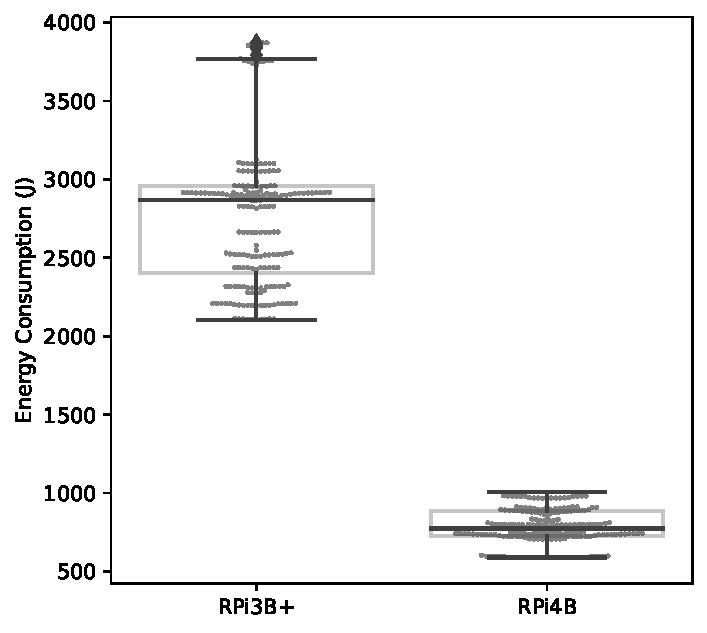
\includegraphics[width=\textwidth]{images/E_per_SUT.pdf}
    \caption{.}
    \label{fig:e_per_sut}
\end{subfigure}
\hspace{\fill}
\begin{subfigure}[t]{0.49\textwidth}
    \centering
    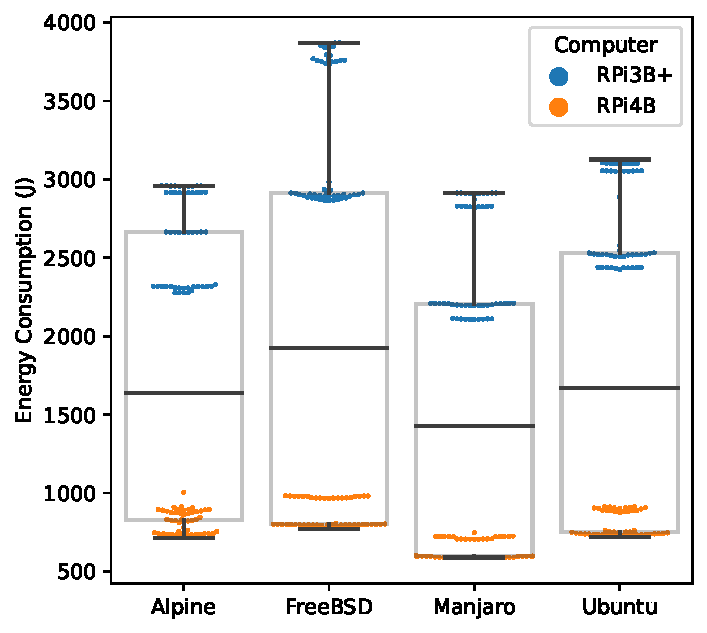
\includegraphics[width=\textwidth]{images/E_per_OS.pdf}
    \caption{.}
    \label{fig:e_per_os}
\end{subfigure}
\hspace{\fill}
\begin{subfigure}{\textwidth}
    \centering
    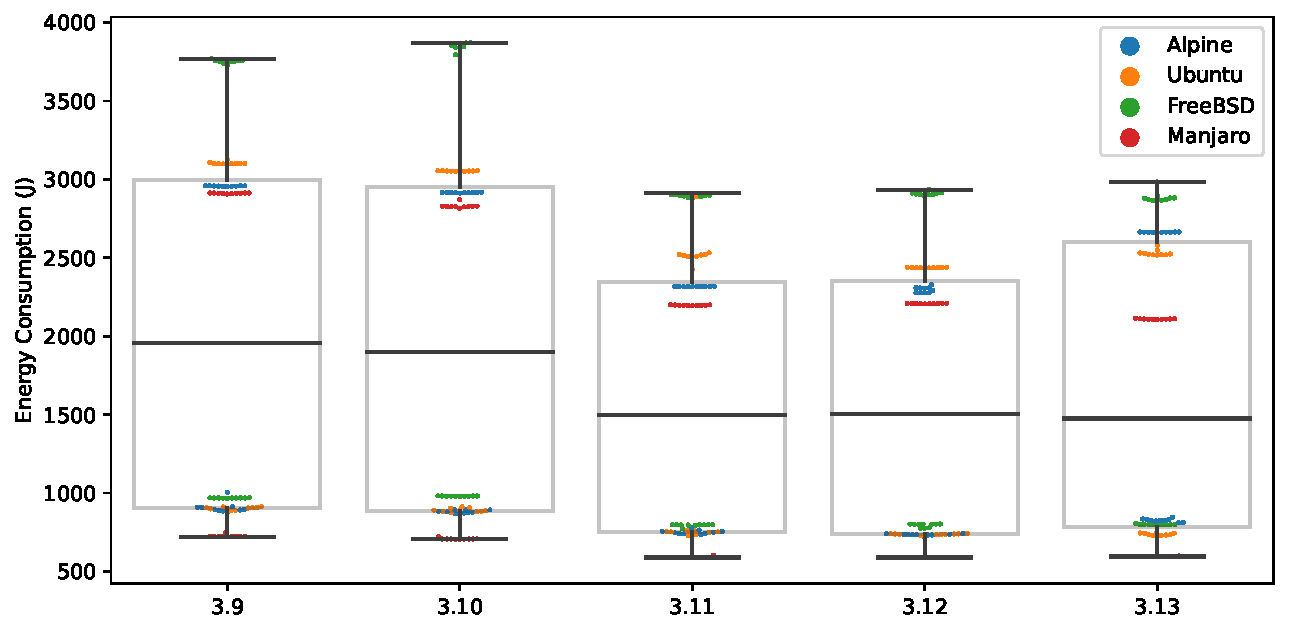
\includegraphics[width=0.9\textwidth]{images/E_per_Python_version.pdf}
    \caption{.}
    \label{fig:e_per_os}
\end{subfigure}
\caption{}\label{fig:e_results}
\end{figure}
\todo{Color dots according to other two features that are not present}



% \begin{figure}[H]
%     \centering
%     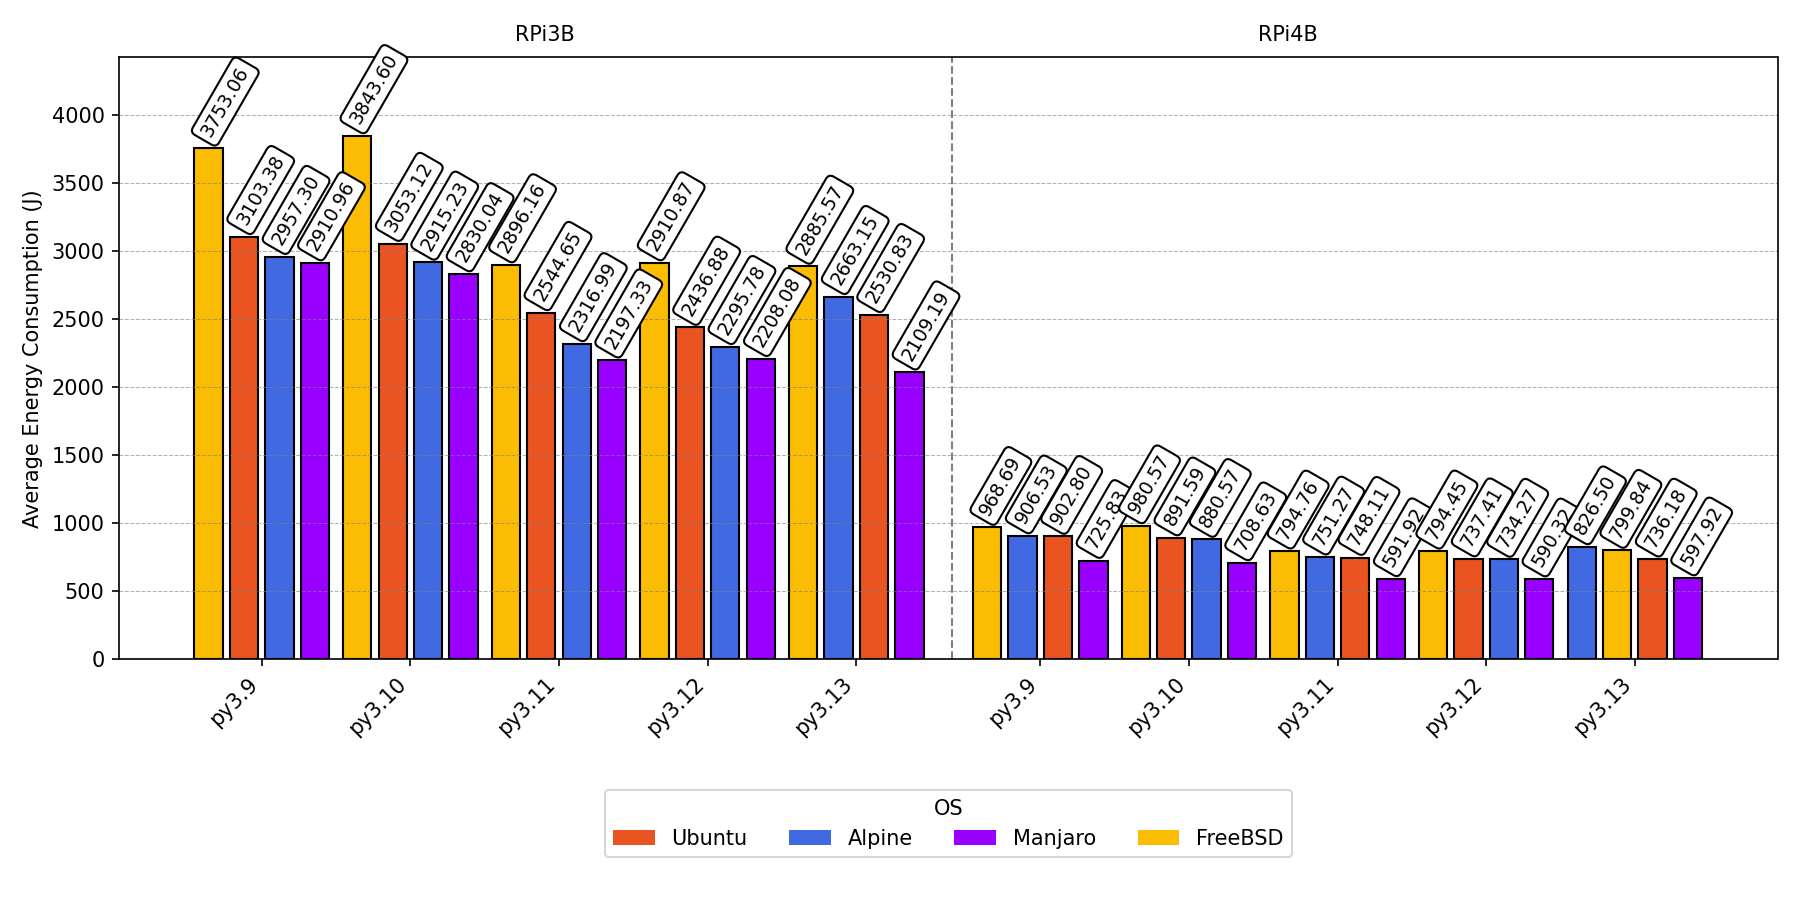
\includegraphics[width=\textwidth]{figures/consumption_barplot_all_pis.png}
%     \caption{Barplot showing the average energy consumption across the 10 recordings made for each configuration.}
%     \label{fig:barplot}
% \end{figure}

% \autoref{fig:barplot} shows the average energy consumption of all benchmarked configurations. The average energy consumption is reflected in both the height of the given column and the label displayed above it. OSs are displayed grouped by Python versions, ordered from lowest to highest version left to right. Within Python version groupings, the OSs are ordered from highest to lowest average energy consumption from left to right. This figure visually indicates, like observed above, RPi3B+ on FreeBSD running Python3.10 having the highest average energy consumption and RPi4B on Manjaro running Python3.12 having the lowest. The figure also clearly indicates a large difference in average energy consumption between the RPi3B+ and RPi4B. A hierarchy between OSs also presents itself, with FreeBSD consistently having the highest energy consumption within a given group (except for Python3.13 on the RPi4B) and Manjaro consistently having the lowest. The hierarchy between Python versions is less clear, but there does seem to be a trend of the higher version having the lower average energy consumption.

% \begin{figure}[H]
%     \centering
%     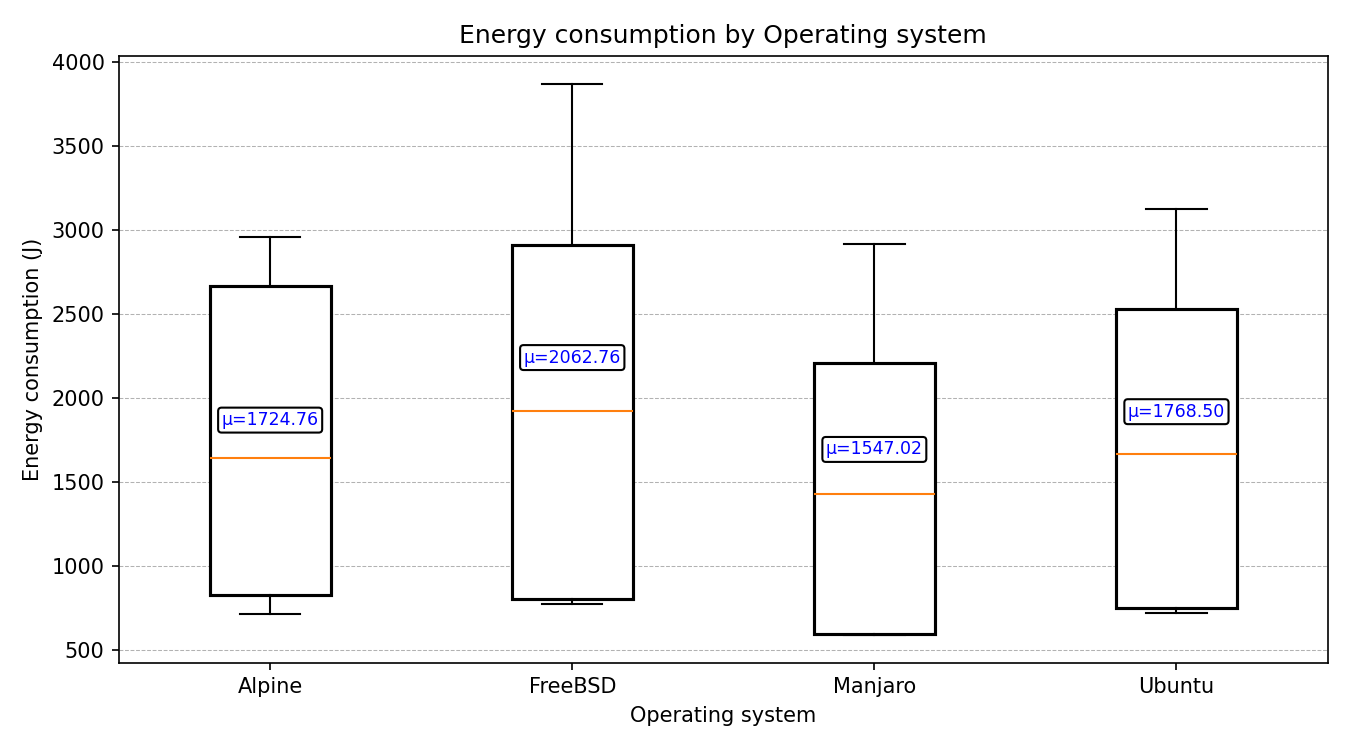
\includegraphics[width=\textwidth]{figures/energy_boxplot_by_os.png}
%     \caption{Boxplot showing the energy consumption of operating systems across all hardware setups and Python versions.}
%     \label{fig:boxplot_os}
% \end{figure}

% \autoref{fig:boxplot_os} shows the energy consumption statistics of OSs across all Python and RPi versions. The minimum is shown by the bottom black line under the white box, the 25th quartile by the bottom of the white box, the median by the orange line, the 75th quartile by the top of the white box, the maximum by the top black bar above the white box and the average ($\mu$) written in blue. These values are extracted from all recordings made for the given OS, such that each box therefore represents 100 individual recordings across 10 configurations. Here we see again a hierarchy of energy consumption, with FreeBSD being highest and Manjaro lowest. We also see an indication that outliers among groups are skewed towards high energy consumption, with the maximum being far removed from the 75th and 25th quartiles. This pattern also indicates that our data for OSs is not normally distributed, but skewed towards the lower end of energy consumption.

% \begin{figure}[H]
%     \centering
%     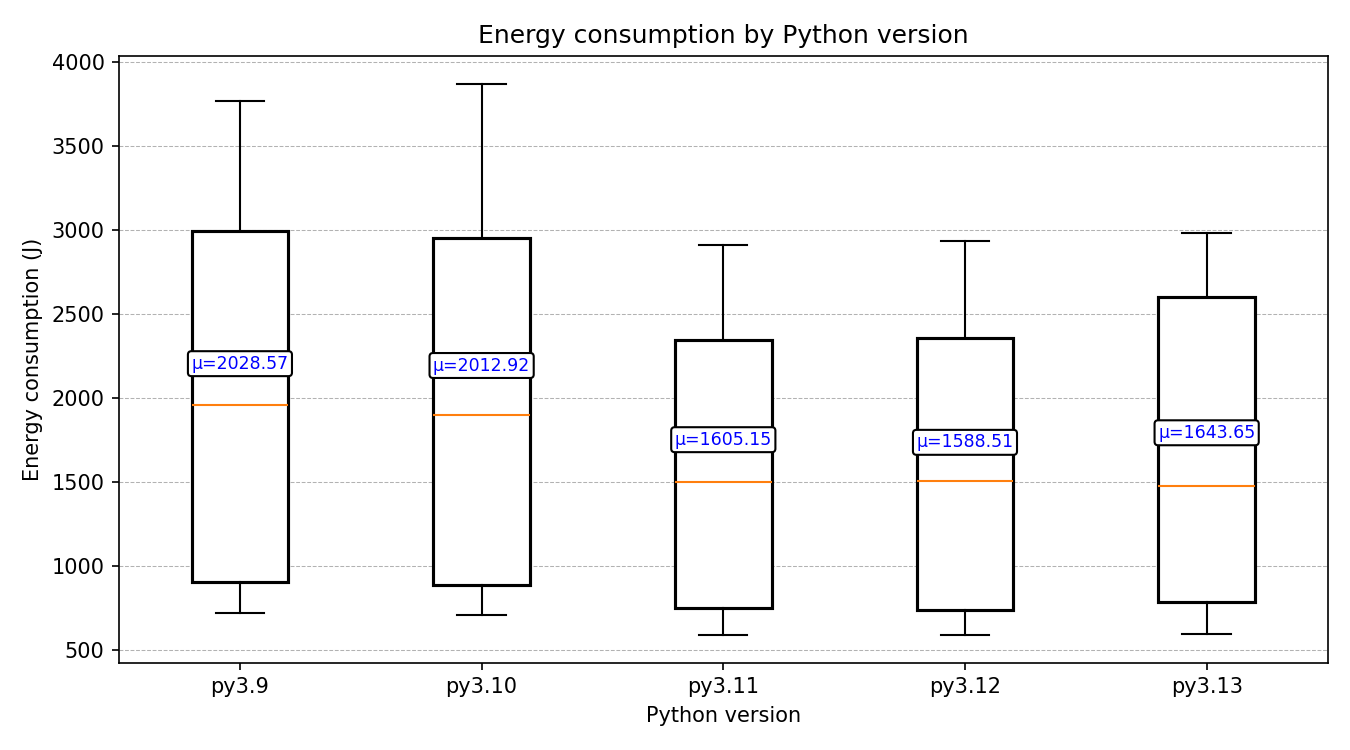
\includegraphics[width=\textwidth]{figures/energy_boxplot_by_python.png}
%     \caption{Boxplot showing the energy consumption of Python versions across all hardware setups and operating systems.}
%     \label{fig:boxplot_python}
% \end{figure}

% \autoref{fig:boxplot_python} shows the energy consumption statistics of Python versions across all operating systems and RPi versions in the same way \autoref{fig:boxplot_os} did for operating systems. These values are accordingly extracted from all recordings made for the Python version, such that each box represents 80 individual recordings across 8 configurations. The hierarchy between Python versions is less clear, but there seems to be a clear decrease in energy consumption from Python3.11 onwards. This data also seems to be skewed towards lower energy consumption, but not as heavily as for OSs. Interestingly, while the values for Python3.11 and 3.12 seem almost equal, the values for Python3.13 seem to be shifted slightly upward, indicating higher energy consumption relative to versions 3.11 and 3.12.

% \begin{figure}[H]
%     \centering
%     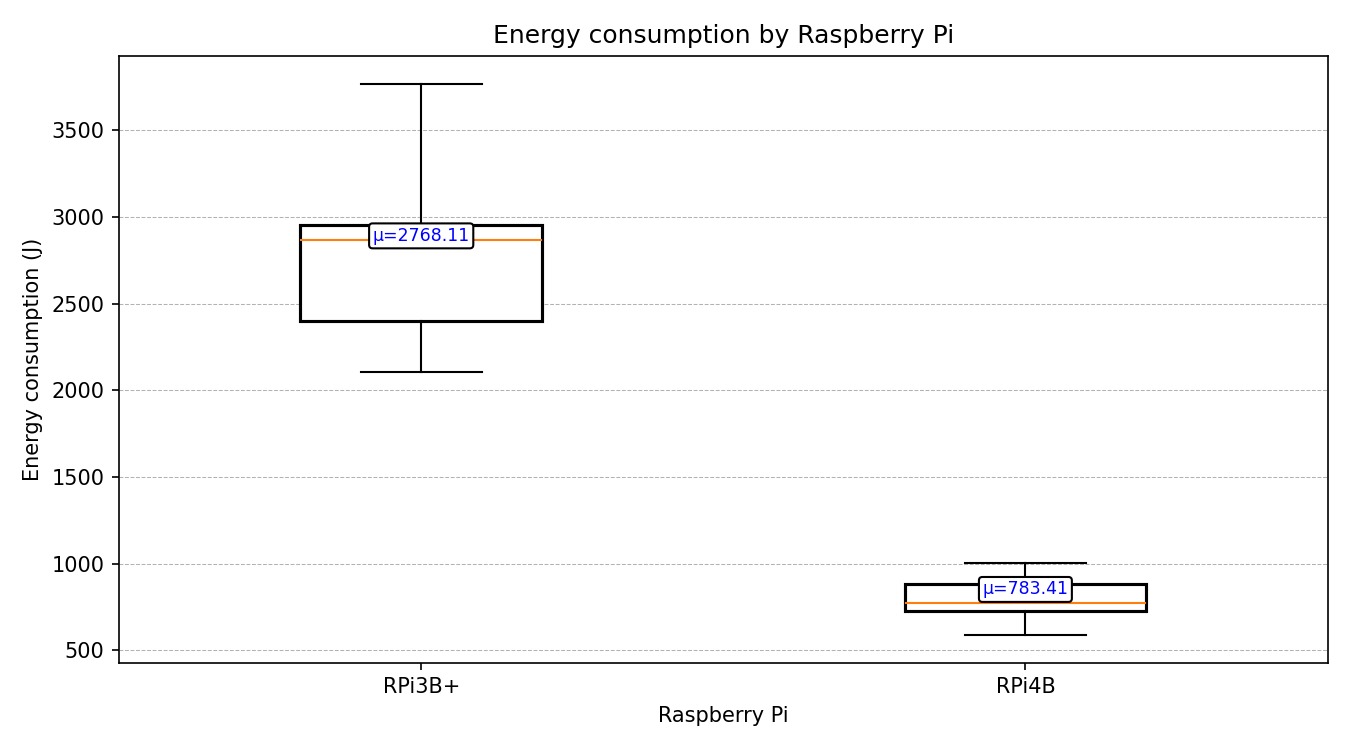
\includegraphics[width=\textwidth]{figures/energy_boxplot_by_rpi.png}
%     \caption{Boxplot showing the energy consumption of RPi versions across all OSs and Python versions.}
%     \label{fig:boxplot_rpi}
% \end{figure}

% \autoref{fig:boxplot_rpi} shows the same statistics as \autoref{fig:boxplot_os} and \autoref{fig:boxplot_python} for the two RPi versions. Each box therefore represents values extracted from 200 individual recordings across 20 configurations. The hierarchy between the two RPis here is readily apparent, with the RPi3B+ having higher energy consumption across the board. The RPi3B+ at first glance seems to have a much higher spread of values, but with recordings ranging from 2000J to well above 3500J compared to a range of just above 500J to around 1000J for the RPi4B, both RPis see just under a doubling in energy consumption from lowest to highest. Both RPis also display a quite balanced range, with only the RPi3B+ being slightly skewed towards lower energy consumption.
